% Hinh 1: giao thuc kiem toan. Hai nhanh do DOC LAP, chi gap nhau o buoc cuoi.
% Quy uoc lay tu paper-lab/transaction-figure-kit/flow/txstyle.tex: nen xam rat nhat,
% MOT mau accent duy nhat, hop goc gan vuong, net 0,5-0,8pt deu, khong bong khong gradient,
% luong du lieu = net lien, nhom = vung net dut kem nhan small-caps.
\documentclass[tikz,border=2pt]{standalone}
\usepackage[T1]{fontenc}
\usepackage[utf8]{inputenc}
\usepackage{times}
\usetikzlibrary{positioning,arrows.meta,fit,backgrounds,calc}

\definecolor{accent}{HTML}{D55E00}
\definecolor{inkgray}{HTML}{3A3F47}

\tikzset{
  bx/.style   = {draw=inkgray,line width=0.6pt,rounded corners=1pt,fill=white,
                 align=center,inner sep=4pt,font=\footnotesize,text width=38mm,minimum height=8mm},
  acc/.style  = {bx,draw=accent,line width=0.9pt},
  src/.style  = {bx,fill=black!4,text width=38mm},
  fl/.style   = {-{Stealth[length=4pt]},draw=inkgray,line width=0.6pt},
  grp/.style  = {draw=inkgray,dashed,line width=0.5pt,rounded corners=2pt,inner sep=7pt},
  lb/.style   = {font=\scriptsize\scshape,text=inkgray},
}

%% SINH TU DONG boi figures/make_figures.py. KHONG SUA TAY.
%% Chi ASCII: tep nay duoc nap boi ca main.tex lan cac tep hinh
%% standalone, va mot so tep hinh khong nap inputenc.
\newcommand{\numCoded}{26}
\newcommand{\numDopKaMax}{455.5}
\newcommand{\numDopKaMed}{359.2}
\newcommand{\numDopRate}{5.4}
\newcommand{\numDopRateMax}{16.9}
\newcommand{\numDopS}{35.9}
\newcommand{\numDopSpread}{15.6}
\newcommand{\numDurMax}{285.5}
\newcommand{\numDurMed}{206.0}
\newcommand{\numEvATMOS}{6}
\newcommand{\numEvCHAWGN}{16}
\newcommand{\numEvCHFADING}{8}
\newcommand{\numEvCHGPP}{4}
\newcommand{\numEvCHTRACE}{0}
\newcommand{\numEvDELAY}{8}
\newcommand{\numEvDOPPLER}{11}
\newcommand{\numEvDOPPLERRATE}{0}
\newcommand{\numEvONBOARD}{3}
\newcommand{\numEvPATHLOSSELEV}{9}
\newcommand{\numEvSNRSWEEP}{7}
\newcommand{\numEvVISIBILITY}{3}
\newcommand{\numFsplMax}{6.72}
\newcommand{\numFsplMed}{3.72}
\newcommand{\numFull}{27}
\newcommand{\numFullPct}{58.7}
\newcommand{\numInATMOS}{2}
\newcommand{\numInCHAWGN}{1}
\newcommand{\numInCHFADING}{0}
\newcommand{\numInCHGPP}{0}
\newcommand{\numInCHTRACE}{0}
\newcommand{\numInDELAY}{4}
\newcommand{\numInDOPPLER}{2}
\newcommand{\numInDOPPLERRATE}{0}
\newcommand{\numInONBOARD}{3}
\newcommand{\numInPATHLOSSELEV}{1}
\newcommand{\numInSNRSWEEP}{2}
\newcommand{\numInVISIBILITY}{2}
\newcommand{\numNotFull}{19}
\newcommand{\numOwd}{3.25}
\newcommand{\numPasses}{30,922}
\newcommand{\numPassesStation}{1,978}
\newcommand{\numPop}{46}
\newcommand{\numSats}{1,200}
\newcommand{\numSlew}{0.049}
\newcommand{\numSlewTen}{0.49}


\begin{document}
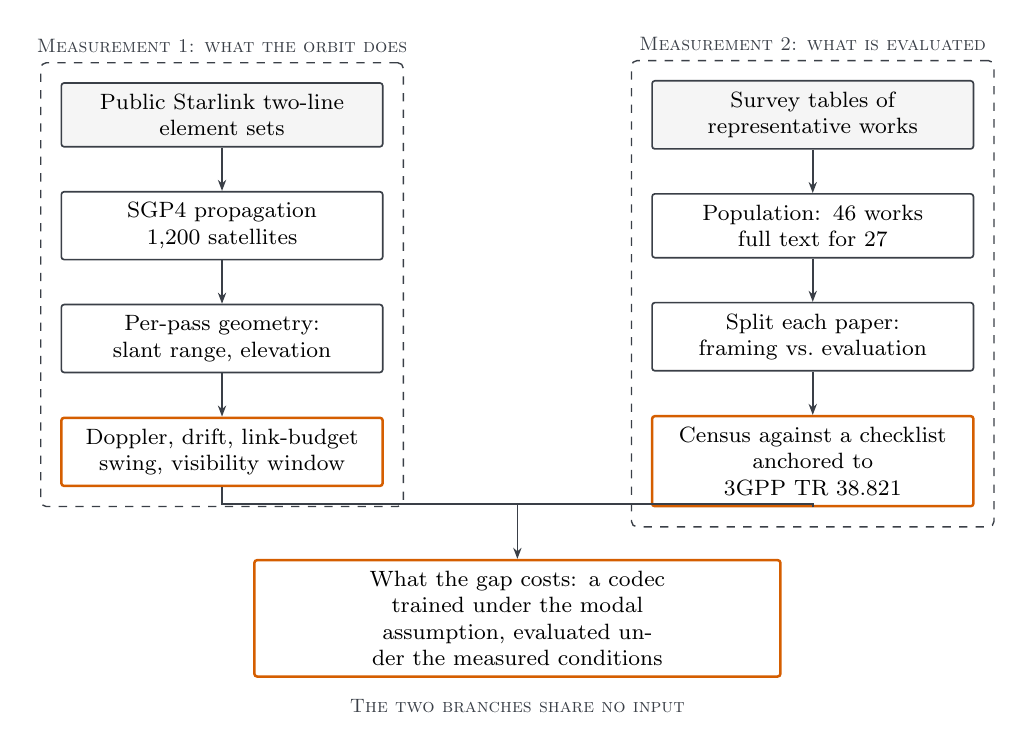
\begin{tikzpicture}[node distance=5.5mm]

% ---------------- nhanh trai: vat ly quy dao ----------------
\node[src] (tle) {Public Starlink two-line\\element sets};
\node[bx,below=of tle] (sgp4) {SGP4 propagation\\\numSats{} satellites};
\node[bx,below=of sgp4] (geom) {Per-pass geometry:\\slant range, elevation};
\node[acc,below=of geom] (dist) {Doppler, drift, link-budget\\swing, visibility window};

% ---------------- nhanh phai: van lieu ----------------
\node[src,right=34mm of tle] (surv) {Survey tables of\\representative works};
\node[bx,below=of surv] (pop) {Population: \numPop{} works\\full text for \numFull{}};
\node[bx,below=of pop] (split) {Split each paper:\\framing vs.\ evaluation};
\node[acc,below=of split] (cens) {Census against a checklist\\anchored to 3GPP TR 38.821};

% ---------------- diem gap ----------------
\node[acc,below=13mm of $(dist)!0.5!(cens)$,text width=64mm] (cost)
     {What the gap costs: a codec trained under the modal\\
      assumption, evaluated under the measured conditions};

\foreach \a/\b in {tle/sgp4, sgp4/geom, geom/dist, surv/pop, pop/split, split/cens}
  \draw[fl] (\a) -- (\b);
% ⛔ Ba lenh -| long nhau truoc day ve ra mot net thua va MOT MUI TEN CHI NGUOC vao khung
%    net dut. Thay bang mot diem hop luu tuong minh: hai nhanh chay xuong gap nhau o (j),
%    roi DUNG MOT mui ten di vao hop.
\coordinate (j) at ($(cost.north)+(0,7mm)$);
\draw[draw=inkgray,line width=0.6pt] (dist.south) |- (j);
\draw[draw=inkgray,line width=0.6pt] (cens.south) |- (j);
\draw[fl] (j) -- (cost.north);

% ---------------- nhom ----------------
\begin{scope}[on background layer]
  \node[grp,fit=(tle)(dist),label={[lb]above:Measurement 1: what the orbit does}] {};
  \node[grp,fit=(surv)(cens),label={[lb]above:Measurement 2: what is evaluated}] {};
\end{scope}

\node[lb,below=1.5mm of cost] {The two branches share no input};

\end{tikzpicture}
\end{document}
